\chapter{Sistemas de Recomendação}
\label{cap:recsys}

A Internet disponibiliza um enorme volume de informação para o usuário, o que cria um desafio pela busca de informação. Por esse problema, empresas cresceram construindo sistemas de recuperação e filtragem, para superação da sobrecarga de informação, como é o caso do Google\footnote{https://www.google.com}. Neste capítulo será apresentado um panorama sobre SR, introduzindo os principais conceitos, tarefas e processos que o caracterizam.

\section{Histórico}
Em razão da crescente dificuldade de usuários administrar a quantidade de informação, é comum decidir baseado em opiniões e recomendações de outros, especialmente quando há pouca experiência no assunto \citep{Resnick:1997:RS:245108.245121}. Conforme mais se expandia a tendência do uso de meios digitais de comunicação, mais rapidamente pessoas migraram de cartas para e-mails. A grande quantidade de e-mails acabava deixando o usuário imerso em documentos, dificultando o consumo do conteúdo. Em 1992, Xerox Palo Alto Research Center apresentou o sistema Tapestry \citep{Goldberg:1992:UCF:138859.138867} na revista mensal ACM Communications\footnote{https://cacm.acm.org/}, como proposta para lidar com o problema quantidade de e-mails. 

O objetivo do sistema era prover listas de e-mails permitindo a inscrição dos usuários naquelas que fossem mais importantes. Alguns sistemas daquela época suportavam filtragem de e-mails baseado no seu conteúdo, mas os autores acreditavam que uma maneira mais eficiente seria com ajuda da avaliação de outros usuários. Interessante ressaltar que o termo “filtragem colaborativa” apresentado no artigo tornou-se comum, e só alguns anos depois surgiu a defesa do termo sistemas de recomendação, mais genérico, como defende \cite{Resnick:1997:RS:245108.245121} em seu artigo.

O sistema do Tapestry foi concebido para a filtragem colaborativa, onde colaborações de outras pessoas auxiliam a outros filtrarem, gravando suas avaliações dos itens. Uma das vantagens da aplicação da filtragem colaborativa é que não depende da análise do conteúdo o que é especialmente útil para a análise itens complexos como vídeos, amplamente usado em serviços como o YouTube\footnote{https://www.youtube.com}. Um exemplo das recomendações no YouTube é na página “em alta” que mostra os vídeos em alta tendência baseada no feedback e visualizações. Em geral, as recomendações personalizadas são dispostas como uma lista de itens ranqueados. O termo “item” é o mais comum a ser denotado por SR para usuários, o que pode designar para diversos tipos, como filmes, livros, músicas etc. 

\begin{figure}
	\centering
	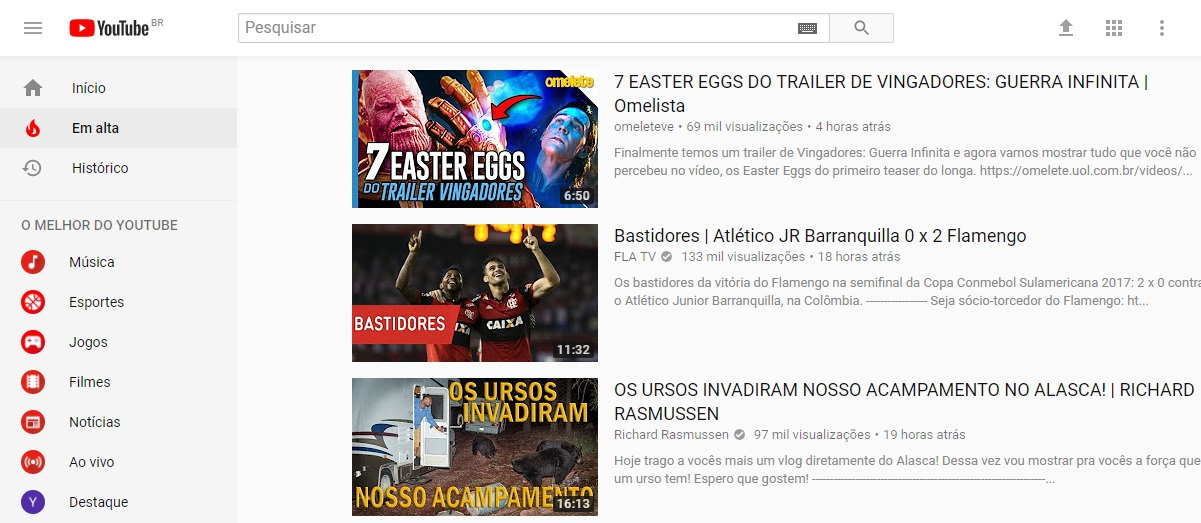
\includegraphics[scale=0.50]{imagens/youtube.jpg}
	\caption{Exemplo de lista de vídeos em alta no YouTube (2017)}
	\label{fig:youtube_em_alta}
\end{figure} 

Para construir o ranque os SRs tentam predizer qual é o item mais adequado àquele usuário \citep{Ricci2011}. Para realizar a tarefa o SR coleta dos usuários suas preferências que podem ser informadas de forma explícita, como avaliação de produtos, ou implícita interpretando suas ações como o histórico de navegação. O princípio do SR é da dependência existente entre o usuário e sua atividade em torno dos itens \citep{Aggarwal:Intro:2016}. Como exemplo, se um usuário comprou um filme de ficção científica, é mais provável que também tenha interesse em outro filme de ficção científica. Dessa forma, o sistema lida com o problema da sobrecarga por filtrar itens que sejam menos prováveis do usuário gostar, baseando-se nas demonstrações do interesse prévio em outros itens, seja por outros usuários ou não.

O aumento da importância da Web como meio eletrônico, especialmente para o e-commerce, também se mostrou como força para o desenvolvimento de sistemas de recomendação.  Na Web o usuário pode informar o seu feedback de produtos sobre o que gostou ou não. Nesse contexto, a aplicação do SR não somente beneficia o usuário, mas também para aqueles que o provem \citep{ ISINKAYE2015261}. Estudos \citep{Mykolas:2015a} demonstram que usuários optam por realizar compras online para poupar tempo. Contudo, com a explosão da variedade de informação disponível, em vez de agir em benefício começa a denigrir a experiência, diminuindo a experiência de uso. É bem aceito que ter escolha é bom, mas ter mais nem sempre é melhor \citep{Ricci2011}.

É importante ressaltar que por fornecer uma informação individualizada, que esteja mais alinhada com o perfil do usuário é o que diferencia os sistemas de recomendação de sistemas de recuperação de informação. Tradicionalmente o motor de buscas deve retornar tudo correspondente a um termo de pesquisa, porém cada vez mais o usuário entra no fator desses sistemas \citep{Burke:2002:HRS:586321.586352}. Sistemas como o Google\footnote{https://www.google.com}, vão além de retornar termos que batem com a consulta, mas também com a quantidade de outras páginas referentes, histórico de buscas, localização, compatibilidade com dispositivos móveis, além de introduzir informações extra a busca, com os quadros do knowledge graph\footnote{ https://www.google.com/intl/bn/insidesearch/features/search/knowledge.html}.

\section{Conceitos}
\label{sec:conceitosSistemaRecomendacao}

Sistemas de recomendação são sistemas de processamento de informação que lidam com diversos tipos de dados para construir recomendações que tentam prever a preferência do usuário \citep{Ricci2011}.  Os dados tratam-se de basicamente de itens que serão apresentados a usuários na forma de recomendações. Técnicas de recomendação variam com dependência do tipo de conhecimento que pode ser extraído de um dado \citep{Ricci2011}. Dados de avaliações possuem pouca informação, o que resulta em técnicas diferentes em relação daquelas que dependem mais da descrição de um item ou relações com as atividades do usuário. Generalizando, SRs referem-se a três tipos de objetos: itens, usuários e transações que são as relações entre usuários e itens.

\begin{itemize}
	\item{\textbf{Itens}: Objetos que são recomendados. Podem ser caracterizados pela complexidade valor ou utilidade. O valor de um item pode ser positivo se é útil para o usuário, ou negativo se não é apropriado ou foi uma decisão errada de seleção por parte do mesmo. O usuário pode ser modelado e representado de diferentes formas, variando bastante em relação do domínio operado pelo SR. Toda vez que um usuário interage com um item constrói-se um custo cognitivo, o que pode entrar na relevância na construção do sistema, mesmo se o usuário não chega a adquirir o item interagido. Alguns exemplos de itens são: livros, notícias (baixa complexidade), computadores, viagens, vagas de trabalho (alta complexidade).}

	\item{\textbf{Usuários}: Usuários de um SR, podendo ter uma variedade de objetivos e características. São explorados uma série de informações variadas para personalizar as recomendações. A informação pode ser estruturada de diversas formas de acordo com o seu tipo, e a seleção de um modelo depende das técnicas a serem utilizadas. Modelos para sistemas de filtragem colaborativa pode usar apenas listas de avaliações de itens por usuários. O modelo de usuário cria o seu perfil, ou seja, armazena suas preferências e necessidades. Usuários também podem ser descritos baseados num padrão de comportamento, como o histórico de navegação na Web sua ou localização.}

	\item{\textbf{Transações}: Genericamente refere-se a transações gravadas das interações entre usuários e o SR. Transações podem ser vistas como um histórico de registros, um log de dados que armazena importantes informações geradas das interações com o sistema. Um registro pode conter a descrição do que foi consultado para uma recomendação particular de um item.}
\end{itemize}

\section{Tarefas de um Sistema de Recomendação}
\label{sec:tarefasSistemaRecomendacao}

Sistemas de recomendação são vistos como mais do que uma ferramenta de prover sugestões de itens que o usuário possa desejar. \citep{Ricci2011} em seu artigo introduziu uma série de funções que podem ser aplicadas a SRs.

\begin{itemize}
	\item{\textbf{Aumento do número de itens vendidos}: Uma das funções mais importantes para aplicações comerciais. O objetivo é ser capaz de vender outros itens comparados àqueles que são vendidos sem qualquer tipo de recomendação. O objetivo é geralmente alcançado devido a itens que são prováveis de serem úteis a necessidade do usuário.}

	\item{\textbf{Vender itens mais diversos}: Também outra função de alta importância, na qual permite o usuário a selecionar itens que podem ser difíceis de encontrar. Num serviço de recomendações de filmes, como o Netflix\footnote{https://www.netflix.com}, o provedor estará interessado que os usuários encontrem conteúdos diversos, não somente os mais populares.}

	\item{\textbf{Aumentar a satisfação do usuário}: Quando um usuário encontra recomendações que sejam de seu interesse, impacta na experiência com o sistema. Um SR bem desenvolvido permite uma combinação precisa de recomendações que juntos a uma interface com boa operabilidade, pode aumentar a noção subjetiva da avaliação de um sistema.}

	\item{\textbf{Aumentar a fidelidade}: Um usuário costuma ser leal a um site que, quando visitado, o reconhece como um consumidor reincidente e o trata como um visitante de valor. É muito como para um SR levar em consideração as informações obtidas em prévias interações com o usuário. Consequentemente, por quanto mais tempo o usuário interage com o site, mais refinado seu modelo torna, ficando cada vez mais efetivo e customizado o resultado da recomendação.}

	\item{\textbf{Melhor entendimento do que o usuário quer}: Outra função importante, na qual pode ser influenciada por outras aplicações, é a descrição das preferências do usuário, seja coletada de forma explícita ou prevista pelo sistema. Um serviço pode decidir reutilizar esses dados do usuário para anunciar um produto em específico, derivado da coleta das informações de transações do SR.}
\end{itemize}

Usuários também podem desejar um SR quando oferece suporte a suas tarefas ou objetivos. \cite{Herlocker:2004:ECF:963770.963772} é uma clássica referência no assunto, e define onze tarefas comuns que SR podem ajudar a implementar. 

\begin{itemize}
	\item{\textbf{Encontrar bons itens}: Recomendar a usuários alguns itens em ranque, junto a uma predição de o quão o usuário possa gostar deles. Também comum no uso em sistema comerciais.}

	\item{\textbf{Encontrar todo os bons itens}: Recomendar todos os itens que satisfazem as preferências do usuário. Neste caso é insuficiente apenas encontrar alguns bons itens. Esta função torna-se útil quando existe um número reduzido de itens, ou quando há uma razão crítica para fornecer informação, como em contextos de uso médico ou financeiro.}

	\item{\textbf{Anotações em contexto}: Dado um contexto, enfatizar alguns itens de uma lista a depender das preferências do usuário.}

	\item{\textbf{Recomendar uma sequência}: Recomendar uma sequência de itens invés de gerar uma única recomendação.}

	\item{\textbf{Recomendar um grupo}: Sugerir grupos de itens bem relacionados que possam ser da preferência do usuário.}

	\item{\textbf{Apenas navegando}: Mesmo que o usuário não possua a intenção de comprar um item, o SR deverá ajudá-lo a navegar pelos catálogo de maneira que encaixe no escopo de interesse do usuário.}

	\item{\textbf{Encontrar um sistema de recomendação confiável}: Nem todos os usuários podem confiar no sistema, dessa forma é importante oferecer testes de suas funcionalidades.}

	\item{\textbf{Melhorar o perfil}: Relativo a capacidade de o usuário prover dados ao SR sobre suas preferências. Tarefa fundamental para personalizar o sistema, caso contrário apenas seria possível oferecer recomendações que fosse relativa ao usuário comum.}

	\item{\textbf{Expressar-se}: Usuários podem não se importar com as recomendações, mas o sistema pode permiti-lo a contribuir com as avaliações e expressão de suas opiniões.}

	\item{\textbf{Ajudar outros}: Para alguns é importante contribuir com informações de suas opiniões e avaliações, pois compartilhando sua experiência pode ajudar outros formarem uma opinião.}

	\item{\textbf{Influenciar outros}: Alguns usuários podem ter apenas o objetivo de influenciar outros, ou até usar o SR para denegrir a imagem de alguns itens.}
\end{itemize}

\section{Técnicas de Recomendação}
\label{sec:tecnicnasRecomendacao}

As recomendações utilizadas no sistema são alcançadas através de algumas técnicas que possuem o objetivo de prever informações sobre itens e preferências de usuários. O SR irá produzir recomendações individualizadas como saída, ou será capaz de guiar o indivíduo de forma personalizada a modo de encontrar itens úteis \citep{Burke:2002:HRS:586321.586352}. Apresentadas não somente como técnicas de filtragem colaborativa, \cite{Resnick:1997:RS:245108.245121}, introduz o termo mais genérico de sistema de recomendação, uma vez que tais sistemas podem explicitamente não utilizar recipientes que talvez sejam desconhecidos uns aos outros. 

Para alcançar as principais funções de um SR, é necessário que o sistema seja capaz de identificar que itens possuem alguma utilidade para o usuário \citep{Ricci2011}. O sistema deve prever ou comparar a utilidade de itens, para decidir como recomendá-los. Dessa forma, as recomendações podem variar conforme os dados conhecidos de usuários e itens, podendo ter maior ou menor influência em uma função específica. Como exemplo, durante a etapa da predição pode ser considerado uma informação que não seja necessariamente personalizada, como apenas recomendar itens mais populares. De posse de poucas informações, ou não conclusivas, a premissa é basear-se num item que tem boa aceitação, ou seja, que é útil para muitos, com uma recomendação provável ao usuário genérico.

Ampliando ao já apresentado Tapestry\citep{Goldberg:1992:UCF:138859.138867}, nem todas as técnicas precisam ser baseadas nas informações de preferências de outros usuários. Na literatura já foram discutidos diversas técnicas, como as apresentadas nos trabalhos de \citep{Ricci2011} e  \citep{ Burke:2002:HRS:586321.586352}. Dentre essas abordagens estão:

\begin{itemize}
	\item{\textbf{Filtragem Colaborativa}: O sistema agrega avaliações ou recomendações, reconhecendo características comuns entre usuários baseando-se nos itens de suas avaliações.}

	\item{\textbf{Baseada em conteúdo}: Objetos de interesse são definidos pela associação de suas características. O sistema aprende e recomenda itens similares ao que usuário demonstrou interesse no passado.}

	\item{\textbf{Demográfico}: Objetivam categorizar o usuário baseado nas informações pessoais dos usuários. Recomendações são baseadas nas classes demográficas dos usuários.}

	\item{\textbf{Baseada em conhecimento}: Realizam sugestões de itens baseadas em inferências das preferências do usuário.}
\end{itemize}

Abaixo será apresentado em maiores detalhes o funcionamento das técnicas de filtragem colaborativa e baseada em conteúdo.

\subsection{Filtragem Colaborativa}

Recomendação com \ac{CF} é uma das técnicas mais familiares e já implementadas \citep{Ricci2011}. A similaridade das preferências e desejos de dois usuários é calculada baseada na similaridade do histórico de avaliações dos usuários. A premissa do método é de que a opinião de outros usuários pode ser selecionada e agregada de forma a prover predições razoáveis ao usuário alvo \citep{HCI-009}. Como exemplo, intuitivamente assume-se que usuários que concordam sobre a qualidade de um filme que João gosta, então João provavelmente gostará de outros filmes que outros usuários avaliaram, mas não assistiu.

O perfil de um usuário na CF pode ser continuamente aprimorado conforme o usuário interage com sistema, podendo levar o tempo de uso como fator de avaliação. Em alguns casos a avaliação pode ser apenas binária (gostei ou não), ou então de valor real que determina um grau de utilidade. Nesse caso, nas avaliações do usuário, o sistema deverá modelar uma função $R(u,i)$ representado o grau de utilidade do item \textit{i} para o usuário \textit{u}.  Basicamente, a tarefa do sistema é estimar um valor de \textit{R} baseado nos pares de usuário e item. Dessa forma, avaliando os dados dessas predições de \textit{R} para o usuário alvo, o sistema recomendará uma quantidade de itens com as maiores utilidades previstas.

Tipicamente, conforme apresentado por \cite{Burke:2002:HRS:586321.586352}, CF divide-se em dois método principais: vizinhança e baseados em modelo. No método da vizinhança o foco é no relacionamento entre itens ou usuários, conhecidos como de \textit{item-item} ou \textit{usuário-usuário} \citep{Ricci2011}, utilizando informações armazenadas com o tempo. O método aborda modelos através da análise da preferência armazenada das classificações de usuário-item, pela avaliação de outros itens similares. Já o método baseado em modelo é criado diretamente do histórico das avaliações para aprender as preferências do usuário, podendo-se usar uma quantidade diversa de técnicas para o aprendizado, como redes neurais. O objetivo é compreender e extrair das interações usuário-item características de destaque para o sistema, podendo criar classes de preferências dos itens.

\subsection{Filtragem Baseada em Conteúdo}

Ao contrário da filtragem colaborativa, sistemas de recomendação baseados em \ac{CBF}, seleciona itens baseados entre as relações de seus conteúdos e as preferências do usuário. A CBF é uma continuação natural das pesquisas nos sistemas de filtragem de informação, \cite{Burke:2002:HRS:586321.586352}.  O método utiliza-se da intuição de que se o usuário demonstrou interesse em certos itens com determinados atributos, é provável de também ter interesse em outros itens de mesmo atributo ou semelhante. Como exemplo, se João gostou dos filmes com o ator \textit{Tom Cruise}, é provável que vá gostar de outros filmes com o mesmo ator. Os sistemas de CBF foram desenhados para explorar cenários com itens que podem ser descritos com um conjunto de propriedades ou atributos \citep{Aggarwal2016}.

Nessa abordagem, o sistema deverá aprender do perfil do usuário seus interesses baseados na combinação das características presentes nos objetos que ele avaliou ou marcou.  O tipo do perfil utilizado no sistema dependerá do método aplicado. A informação das preferências do usuário pode manifestar-se de forma explícita, onde existem avaliações ou indicações dos itens favoritos, ou de forma implícita como itens que o usuário comprou. Nos métodos aplicados na CBF, as descrições dos itens avaliados são usadas como dados de treinamento para criar uma classificação específica para o usuário \citep{Aggarwal2016}. Os perfis da filtragem baseada no conteúdo são modelos de longo prazo, onde mais dados são atualizados conforme mais evidências do usuário são observadas, \cite{Burke:2002:HRS:586321.586352}.

Apesar da descrição do conteúdo, ou seja, atributos particulares dos itens, sejam o centro da análise da utilidade de novos itens para recomendação, a avaliação de outros usuários tem significativo impacto no sistema \citep{Aggarwal2016}. Essa característica apresenta tanto vantagens como desvantagens. Por um lado, num contexto da \textit{partida a frio}, onde há pouca informação disponível sobre as avaliações dos usuários, há margem de utilização enquanto houver outras suficientes informações das preferências do usuário. Mesmo quando um item é novo ou desconhecido, o sistema ainda pode aproveitar suas características para recomendar novos itens, algo que não é possível apenas baseando-se nas avaliações de outros usuários. 

Assim, sistemas de CBF são tipicamente utilizados quando há suficiente informação das preferências do usuário disponíveis. Particularmente, são de mais fácil utilização quando usados em domínios com dados não estruturados e ricos em textos, como páginas da Web.

%\subsection{Arquitetura de Sistemas de Recomendação Baseados em Conteúdo}
	
\subsection{Comparação das Técnicas de Recomendação}

Todas as abordagens dos SR possuem vantagens e desvantagens, dependendo de questões como novos itens, usuários, e quantidade de informação disponível sobre os dois. Em relação a novos usuários, como recomendações partem da comparação de informações do usuário alvo e outros usuários, quanto menos avaliações o sistema possuir, mais difícil será a classificação. Já para novos itens, o problema surge em domínios em constante atualização e novas informações e onde cada usuário pouco avalia. Também pode ser visto como o problema do \textit{early rater}, uma vez que a pessoa que avalia primeiro, pouco se beneficia.

\cite{Burke:2002:HRS:586321.586352} apresentou alguns pontos comuns das diferenças desses sistemas:

\begin{itemize}
	\item{\textbf{Sistemas baseados em filtragem colaborativa}: Dependem da sobreposição de avaliações através dos usuários e possuem dificuldades quando há escassez dessas avaliações dos itens. O problema ressalta que as técnicas colaborativas melhor servem quando a densidade de interesses de usuários é alta através de um universo de itens que não mudam rapidamente.} 

	\item{\textbf{Sistemas baseados em conteúdo}: Possuem o problema da partida a frio, onde o sistema não acumulou dados suficientes para construir uma recomendação confiável. Também são limitados pela quantidade de informações disponíveis e associadas aos itens. Isto acaba colocando a técnica muito dependente da descrição dos dados. Uma grande desvantagem em relação a abordagem colaborativa é que a abrangência de gêneros, onde deixa o usuário sujeito ao mesmo tipo de conteúdo. A depender da CF, pela a avaliação de outros usuários é possível recomendar itens “fora da caixa”.}
\end{itemize}

\section{Aplicações de Sistemas de Recomendação}

O sistema Tapestry \citep{Goldberg:1992:UCF:138859.138867} foi um marco inicial no desenvolvimento de aplicações, introduzindo a filtragem colaborativa. Hoje, SR são quase que obrigatórios para muitas lojas online e serviços de entretenimento, tornou-se algo comum e já disseminado entre usuários. A seguir será apresentado algumas aplicações em destaque que usam sistemas de recomendação.

\subsection{Netflix}

Com a evolução da Internet, as mídias físicas para consumo de entretenimento começaram a decair, especialmente para filmes. O avanço na conexão da banda larga trouxe o modelo do \textit{streaming}\footnote{Transmissão contínua de mídia pela Internet, (https://directradios.com/streaming)} que possibilita o usuário a assistir o conteúdo a qualquer momento, lugar, sem ter que  necessariamente sair de sua residência para ir à uma locadora, por exemplo. Embora o Netflix\footnote{https://www.netflix.com}, tenha iniciado no ramo de aluguel de \ac{DVD}s \citep{keating2012netflixed}, a companhia rapidamente abandonou este modelo e partiu para a transmissão de filmes e em seguida para produção de seus próprios filmes e séries. Dessa forma, o serviço de filmes e séries cresceu, ocupou espaço das televisões, cinemas e alcançou diversos países.

\begin{figure}
	\centering
	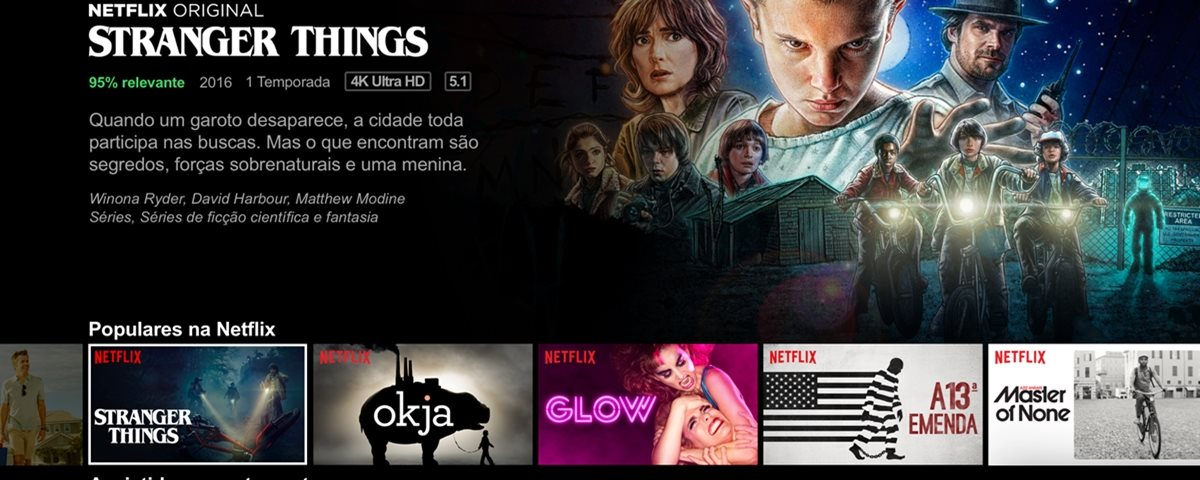
\includegraphics[scale=0.40]{imagens/netflix_recsys.jpg}
	\caption{Recomendação de Filmes no serviço Netflix. Figura elaborada pelo autor (2017).}
	\label{fig:netflix}
\end{figure}

Com a crescente quantidade de títulos disponíveis na plataforma e também de usuários, logo o serviço desenvolveu seu próprio sistema de recomendações de vídeos, baseado nas avaliações de usuários. Em outubro de 2006 a companhia publicou um concurso pelo melhor sistema de filtragem colaborativa que poderia superar a precisão de seu SR, o Cinematch \citep{bennett2007netflix}. Neste ponto o serviço já tinha lançado um banco de dados contendo 100 milhões de avaliações de usuários e 18 mil títulos. O Cinematch analisava as avaliações acumuladas dos usuários semanalmente usando uma variante da correlação de Pearson, com todos os outros filmes para determinar uma lista de filmes similares. Sendo assim, conforme o usuário provia avaliações, o sistema computava uma regressão baseada nessa correlação para determinar uma predição única personalizada. Caso não houvesse nenhuma predição personalizada a média de todas as avaliações é usada. As predições eram apresentadas como conjunto de 5 estrelas.

O desempenho do Cinematch é medido principalmente pelo cálculo da raiz do erro quadrático médio, \ac{RMSE} \citep{Herlocker:2004:ECF:963770.963772}, das predições do sistema contra as avaliações que os usuários informam. Com os sistemas propostos no concurso, a companhia propôs um prêmio para aqueles que conseguissem melhorar a precisão em 10\%. Nesse ano de 2017, a companhia migrou seu sistema de avaliação das tradicionais 5 estrelas para uma avaliação binária, o \textit{Like} e \textit{Dislike} \citep{ VarietyNetflix:2017}. Segundo a companhia, os usuários confundiam a avaliação de 5 estrelas, pois na verdade eram sempre as predições avaliadas para o filme, assim agora as predições aparecem no formato de porcentagem de relevância e a avaliação do usuário é indicada pelos símbolos do gostei ou não gostei. Também as predições passaram a serem baseadas apenas no histórico e comportamento do usuário e não mais na média em relação às outras pessoas.

\subsection{Skoob}

Em janeiro de 2009, o analista de sistemas Lindeberg Moreira realizou sua ideia de criar uma plataforma em que pessoas socializassem o ato da leitura \citep{SkoobSocializando:2009}, o Skoob\footnote{ https://www.skoob.com.br}. O sistema criado trata-se de uma rede social para leitores no Brasil \citep{SkoobQuemSomos:2017}. Na plataforma, o usuário montará uma estante virtual realizando buscas pelos livros e em seguida indicar o que já fez com o livro, se já leu, se lerá ou está relendo. Após a seleção dos livros os usuários poderão avaliar seus livros, podendo até escrever resenhas completas ou de capítulos dos livros, compartilhando com outras pessoas na plataforma.

\begin{figure}
	\centering
	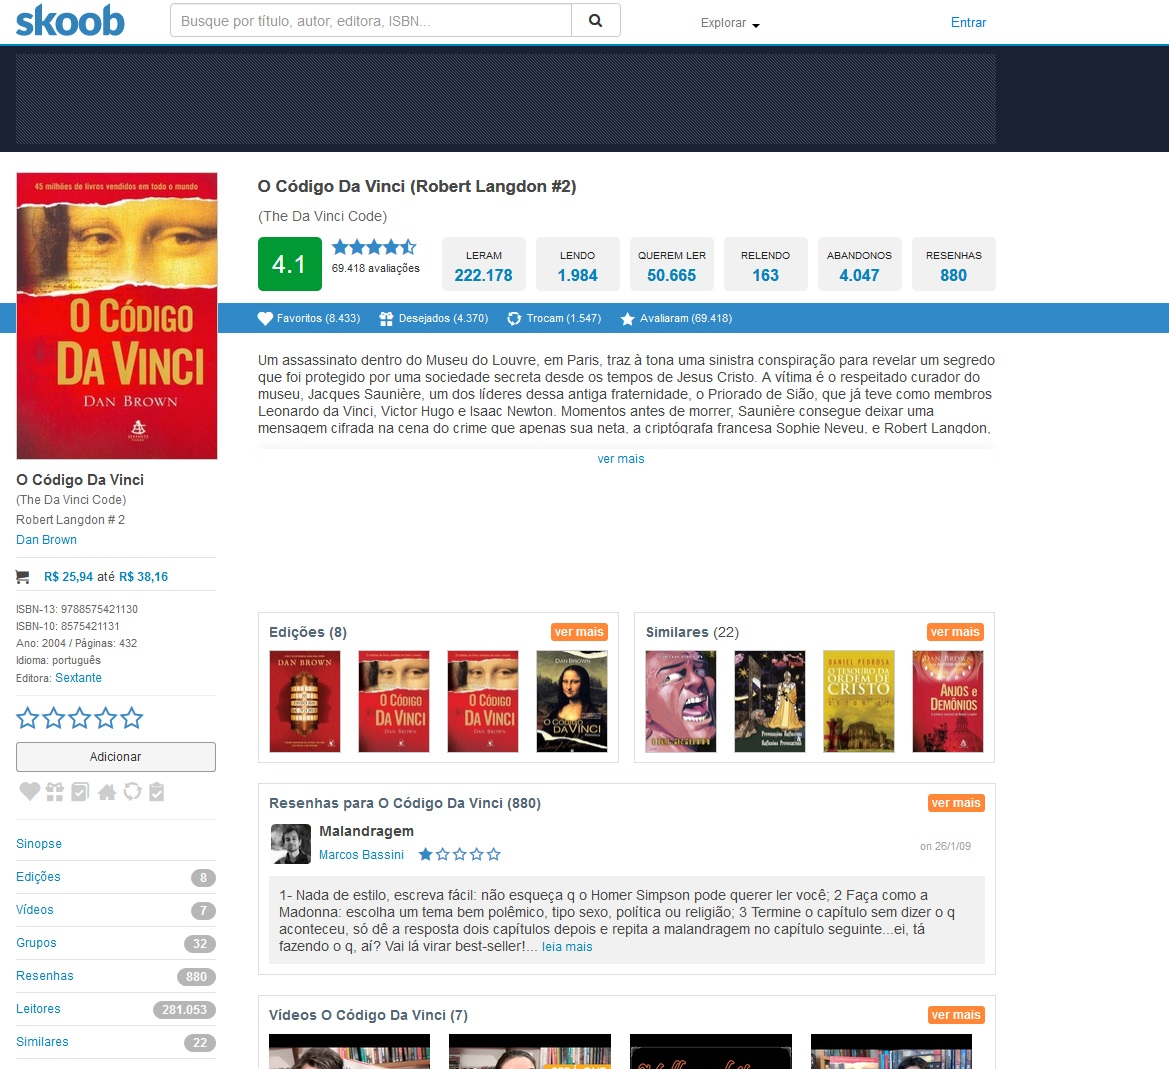
\includegraphics[scale=0.40]{imagens/skoob_recsys.jpg}
	\caption{Página de avaliação do livro no Skoob. Figura elaborada pelo autor (2017).}
	\label{fig:skoob}
\end{figure}

A rede social, conta com algumas mecânicas para ajudar usuários a encontrar livros, com um sistema busca de livros, recomendação com filtragem colaborativa baseada nas avaliações de usuários, dos marcados como mais lidos, lendo, quero ler entre outros. A plataforma também conta com um sistema que indica livros similares. Todos esses processos não somente levam a questão da socialização da leitura e escrita entre indivíduos que compartilham interesses, surgidas a partir da aplicação, mas passam a influenciar a forma como usuários passam a tratar a leitura fora do ambiente da comunidade virtual, é o que aponta \cite{SkoobUFPE:2010}.

\section{Sumário}

Neste capítulo, foi apresentado um panorama geral sobre os sistemas de recomendação. Inicialmente abordando o histórico envolvido e motivações na criação dos conceitos envolvidos do tema. Em sequência foi aprofundado e explicado os conceitos utilizados nesses sistemas. Então, foi apresentado as tarefas e técnicas utilizadas. Também foi aprofundado algumas diferenças e dificuldades entre as principais técnicas de recomendação. Por fim, foi mostrado exemplos de aplicações que utilizam esses sistemas de recomendação. No capítulo \ref{cap:semantic_web} será discutido sobre os conceitos envolvidos na Web Semântica, bem como os princípio dos dados ligados e o serviço da DBPedia\footnote{http://wiki.dbpedia.org}.